\documentclass{article}
\usepackage{geometry}
\geometry{
  a4paper,
  total={170mm,257mm},
  left=20mm,
  top=20mm,
}

\usepackage{fontspec}
\IfFontExistsTF{Poppins}{\setmainfont{Poppins}\setsansfont{Poppins}}{\setmainfont{Latin Modern Roman}\setsansfont{Latin Modern Sans}}
\IfFontExistsTF{Menlo}{\setmonofont{Menlo}}{\setmonofont{Latin Modern Mono}}

\usepackage{graphicx}
\usepackage{fancyhdr}
\usepackage{booktabs}
\usepackage{array}
\usepackage{longtable}
\usepackage{tabularx}
\usepackage{enumitem}
\usepackage[table]{xcolor}
\usepackage{amsmath}
\usepackage{amssymb}
\usepackage{hyperref}
\usepackage{float}
\usepackage{listings}

\definecolor{primary}{HTML}{1D4ED8}
\definecolor{primaryDark}{HTML}{1E3A8A}
\definecolor{accent}{HTML}{F97316}
\definecolor{softBlue}{HTML}{EAF2FF}
\definecolor{softOrange}{HTML}{FFF3E8}
\definecolor{softGreen}{HTML}{ECFDF3}
\definecolor{softPurple}{HTML}{F4F0FF}
\definecolor{textGray}{HTML}{334155}
\definecolor{tableHead}{HTML}{DBEAFE}
\definecolor{codeBg}{HTML}{F8FAFC}

\title{Support Vector Machine: SVC, Hyperplane, Kernel, dan Parameter Tuning}
\author{Danish Rafie Ekaputra}
\date{Week 11 -- Praktikum Data Mining}
\newcommand{\theauthor}{Danish Rafie Ekaputra}
\newcommand{\thedate}{Week 11 -- Praktikum Data Mining}

\fancypagestyle{plain}{%
    \fancyhf{}
    \fancyfoot[L]{\textcolor{textGray}{\thedate}}
    \fancyfoot[R]{\textcolor{primary}{\thepage}}
    \fancyhead[L]{\textcolor{primaryDark}{Praktikum Data Mining}}
    \fancyhead[R]{\textcolor{textGray}{\theauthor}}
    \renewcommand{\headrulewidth}{0.4pt}
    \renewcommand{\footrulewidth}{0.4pt}
}
\pagestyle{plain}

\makeatletter
\def\@maketitle{%
  \newpage
  \null
  \vskip 0.5em%
  \noindent\colorbox{primary}{%
    \begin{minipage}{0.96\textwidth}
      \vspace{1.1em}
      \begin{center}
        {\color{white}\LARGE\bfseries \@title \par}
        \vspace{0.45em}
        {\color{white}\large Materi Week 11 -- Supervised Learning}
      \end{center}
      \vspace{1.1em}
    \end{minipage}}
  \par
  \vskip 1em}
\makeatother

\hypersetup{
    colorlinks=true,
    linkcolor=primaryDark,
    urlcolor=primary,
    citecolor=primaryDark
}

\lstset{
    basicstyle=\ttfamily\small,
    breaklines=true,
    frame=single,
    rulecolor=\color{primary!35},
    columns=fullflexible,
    backgroundcolor=\color{codeBg},
    keywordstyle=\color{primaryDark}\bfseries,
    commentstyle=\color{textGray},
    stringstyle=\color{accent}
}

\newcommand{\code}[1]{\texttt{#1}}
\newcommand{\method}[1]{\textbf{\textcolor{primaryDark}{#1}}}
\newcommand{\sectiontag}[1]{\textcolor{accent}{\textbf{#1}}}
\newcommand{\infobox}[2]{%
  \par\vspace{0.6em}
  \noindent\colorbox{#1}{%
    \begin{minipage}{0.96\textwidth}
    \vspace{0.65em}
    #2
    \vspace{0.65em}
    \end{minipage}}
  \par\vspace{0.8em}
}

\begin{document}

\maketitle

\noindent\begin{tabular}{@{}>{\bfseries}ll}
    Modul & Week 11: Supervised Learning\\
    Topik & Support Vector Machine dan SVC\\
    Penulis & \theauthor\\
    Mata Kuliah & Praktikum Data Mining
\end{tabular}

\section*{Tujuan Pembelajaran}

Setelah mempelajari materi ini, mahasiswa diharapkan mampu:

\begin{enumerate}[leftmargin=*]
    \item Menjelaskan basic concept Support Vector Machine untuk supervised learning.
    \item Menjelaskan hyperplane, margin, dan support vectors.
    \item Membedakan hard margin dan soft margin SVM.
    \item Menjelaskan intuisi convex optimization pada SVM.
    \item Menggunakan konsep dasar Support Vector Classification (SVC).
    \item Menjelaskan kernel trick dan beberapa kernel function umum.
    \item Menjelaskan parameter penting pada SVC seperti \code{C}, \code{kernel}, \code{gamma}, \code{degree}, dan \code{class\_weight}.
    \item Menentukan parameter SVM dengan Grid Search, Random Search, dan Optuna.
\end{enumerate}

\infobox{softBlue}{\textbf{Big idea.} SVM tidak hanya mencari boundary yang memisahkan class. SVM mencari boundary yang punya \textit{margin} paling aman terhadap data terdekat, lalu mengontrol trade-off antara margin besar dan training error melalui parameter \code{C}.}

\section{Positioning: Kenapa SVM?}

Dalam classification, banyak model bisa membuat decision boundary. Pertanyaan utama SVM adalah: dari semua boundary yang mungkin, boundary mana yang paling aman untuk generalization? Jawabannya adalah boundary dengan margin terbesar. Margin besar berarti garis pemisah tidak terlalu dekat dengan data training, sehingga lebih stabil ketika bertemu data baru.

\begin{table}[H]
\centering
\rowcolors{2}{softBlue}{white}
\begin{tabularx}{\textwidth}{>{\bfseries}lXX}
\rowcolor{tableHead}
Kondisi & Kenapa SVM Cocok & Catatan \\
\toprule
High-dimensional features & SVM efektif saat jumlah fitur besar. & Tetap perlu regularization. \\
Dataset kecil-menengah & Kernel SVM bisa menangkap boundary non-linear. & Untuk dataset sangat besar, pertimbangkan LinearSVC. \\
Boundary kompleks & Kernel trick membuat boundary non-linear di input space. & Kernel dan parameter harus dipilih hati-hati. \\
Butuh margin-based classifier & SVM eksplisit maximize margin. & Sensitif terhadap scaling fitur. \\
\bottomrule
\end{tabularx}
\caption{Kondisi yang membuat SVM menjadi pilihan model yang kuat.}
\end{table}

\infobox{softOrange}{\textbf{Practical note.} SVM sangat sensitif terhadap skala fitur. Gunakan \code{StandardScaler} dalam \code{Pipeline} agar scaling hanya di-fit pada training data dan diterapkan konsisten saat cross-validation maupun testing.}

\section{Hyperplane, Margin, dan Support Vectors}

\subsection{Hyperplane}

Hyperplane adalah decision boundary dalam ruang fitur. Pada data 2D bentuknya garis, pada data 3D bentuknya bidang, dan pada dimensi lebih tinggi disebut hyperplane. Formulanya:

\begin{equation}
w^T x + b = 0
\end{equation}

Prediction rule untuk binary classification:

\begin{equation}
f(x) = \operatorname{sign}(w^T x + b)
\end{equation}

Jika nilai fungsi positif, data masuk class positif. Jika negatif, data masuk class negatif.

\subsection{Margin dan Support Vectors}

Margin adalah jarak aman antara hyperplane dan data terdekat dari setiap class. Untuk data linearly separable, lebar margin berhubungan dengan:

\begin{equation}
\text{margin} = \frac{2}{\lVert w \rVert}
\end{equation}

Karena itu, maximize margin setara dengan minimize $\lVert w \rVert^2$. Data points yang berada paling dekat dengan hyperplane disebut \textit{support vectors}. Mereka adalah data yang benar-benar menentukan posisi boundary.

\begin{figure}[H]
\centering
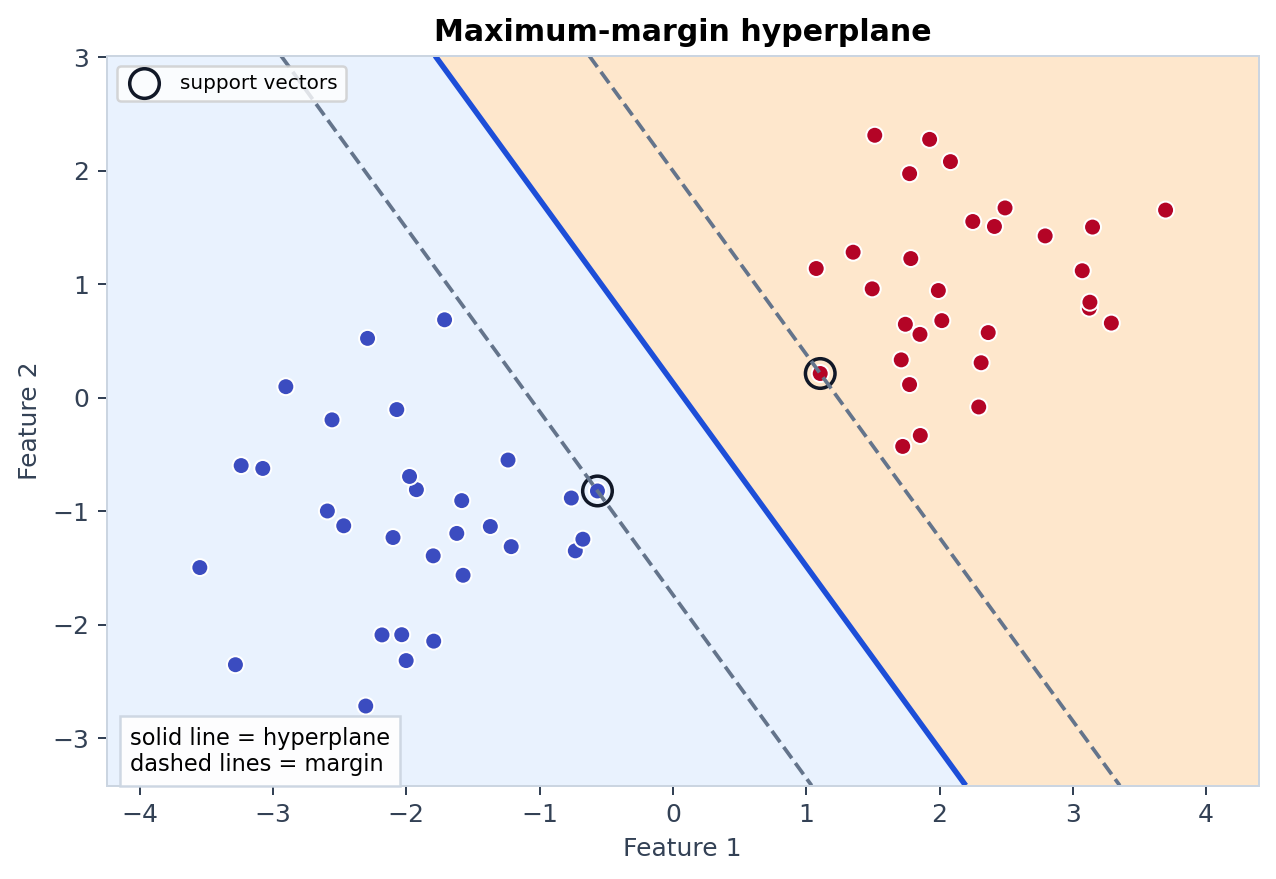
\includegraphics[width=0.82\textwidth]{figures/01_svm_max_margin_hyperplane.png}
\caption{Maximum-margin hyperplane. Garis penuh adalah decision boundary, garis putus-putus adalah margin, dan lingkaran hitam menunjukkan support vectors.}
\end{figure}

\infobox{softGreen}{\textbf{Key insight.} Tidak semua data training punya pengaruh yang sama. Pada SVM, boundary terutama ditentukan oleh support vectors, yaitu data paling dekat dengan margin.}

\section{Hard Margin dan Soft Margin}

\subsection{Hard Margin}

Hard margin mengasumsikan data bisa dipisahkan sempurna tanpa error. Objective-nya:

\begin{equation}
\min_{w,b} \frac{1}{2}\lVert w \rVert^2
\end{equation}

Dengan constraint:

\begin{equation}
y_i(w^T x_i + b) \geq 1
\end{equation}

Hard margin jarang cocok untuk real-world data karena data sering punya noise, overlap, atau outlier.

\subsection{Soft Margin}

Soft margin memperbolehkan sebagian data masuk ke margin atau bahkan salah klasifikasi. Pelanggaran ini diukur dengan slack variable $\xi_i$ dan dikontrol oleh parameter \code{C}.

\begin{equation}
\min_{w,b,\xi} \frac{1}{2}\lVert w \rVert^2 + C \sum_{i=1}^{n}\xi_i
\end{equation}

Subject to:

\begin{equation}
y_i(w^T\phi(x_i)+b) \geq 1-\xi_i, \qquad \xi_i \geq 0
\end{equation}

\begin{table}[H]
\centering
\rowcolors{2}{softOrange}{white}
\begin{tabularx}{0.9\textwidth}{>{\bfseries}lXX}
\rowcolor{softOrange}
Nilai \code{C} & Efek & Risiko \\
\toprule
Kecil & Margin lebih lebar dan lebih toleran terhadap error. & Bisa underfit. \\
Besar & Error dipenalti lebih keras dan boundary mengejar training data. & Bisa overfit. \\
\bottomrule
\end{tabularx}
\caption{Interpretasi parameter \code{C} pada soft-margin SVM.}
\end{table}

\begin{figure}[H]
\centering
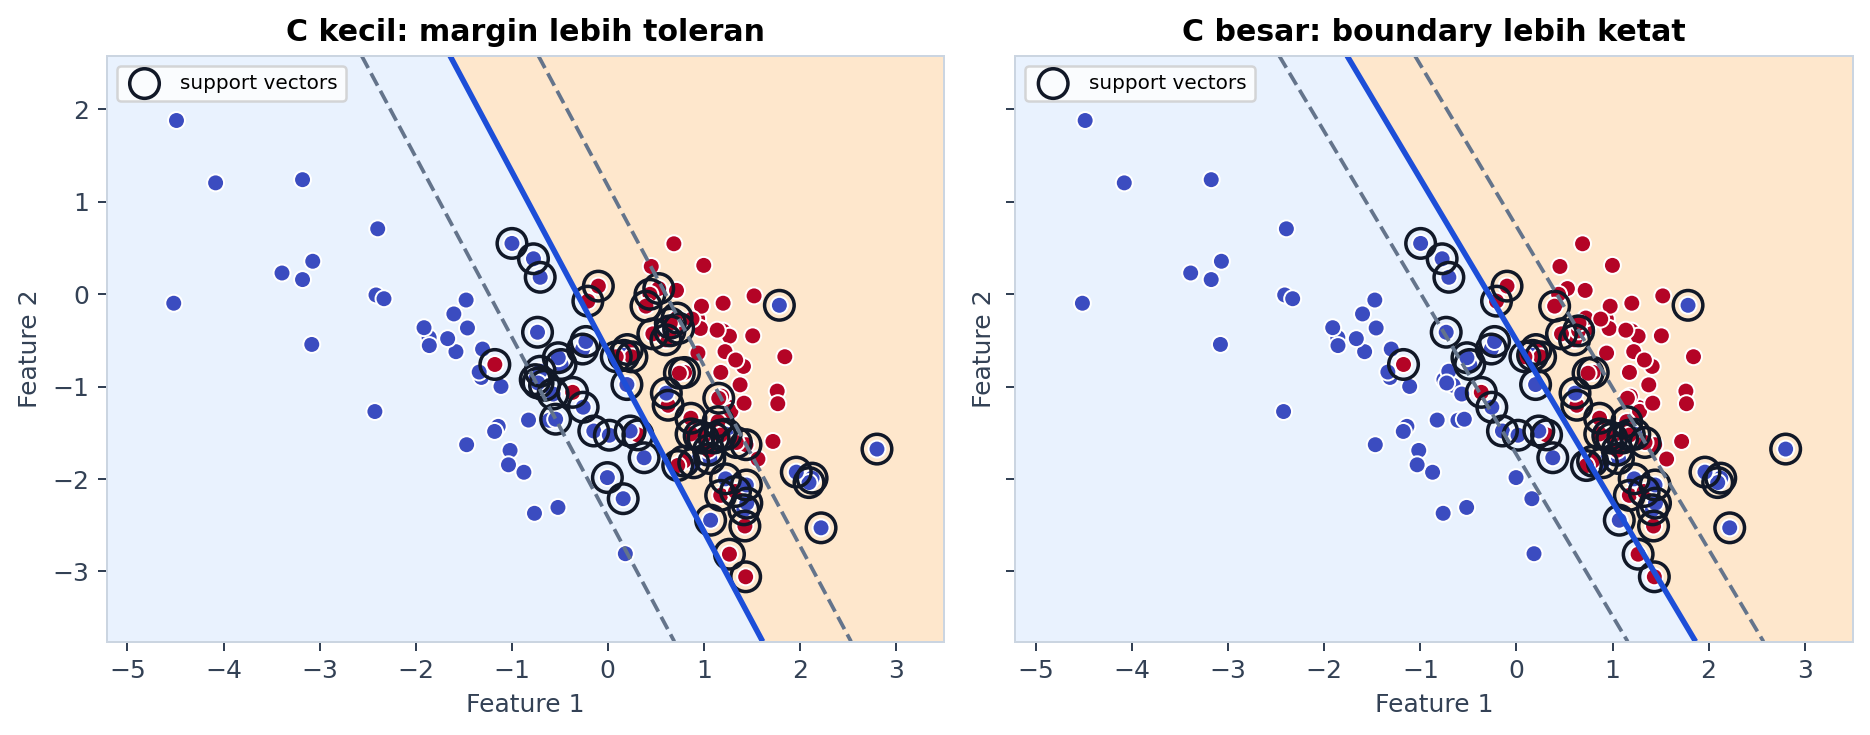
\includegraphics[width=0.98\textwidth]{figures/02_svc_c_effect.png}
\caption{Efek parameter \code{C}. Nilai \code{C} kecil membuat boundary lebih toleran, sedangkan \code{C} besar membuat boundary lebih ketat terhadap training data.}
\end{figure}

\section{Convex Optimization Intuition}

SVM training menyelesaikan optimization problem yang convex. Artinya, objective SVM punya global optimum yang bisa dicari secara stabil. Secara praktis, SVM menggabungkan objective margin dan penalty error.

\begin{table}[H]
\centering
\rowcolors{2}{softGreen}{white}
\begin{tabularx}{\textwidth}{>{\bfseries}lX}
\rowcolor{softGreen}
Komponen Objective & Makna \\
\toprule
$\frac{1}{2}\lVert w \rVert^2$ & Membuat margin besar dan model lebih sederhana. \\
$C\sum \xi_i$ & Penalize data yang melanggar margin atau salah klasifikasi. \\
\bottomrule
\end{tabularx}
\end{table}

Soft-margin linear SVM juga dapat dilihat melalui hinge loss:

\begin{equation}
\ell_i = \max(0, 1 - y_i(w^T x_i + b))
\end{equation}

Jika point benar dan jauh di luar margin, loss bernilai 0. Jika point berada di dalam margin atau salah klasifikasi, loss menjadi positif.

\infobox{softPurple}{\textbf{Teaching intuition.} SVM bukan model yang sekadar ``mencari garis''. Ia menyelesaikan masalah optimasi: cari boundary paling sederhana dengan margin besar, tetapi tetap mengontrol training mistake.}

\section{Support Vector Classification}

\subsection{SVC di scikit-learn}

\code{SVC} adalah implementasi Support Vector Classification berbasis LIBSVM. Ia mendukung binary classification, multiclass classification, kernel linear maupun non-linear, dan class weighting untuk imbalanced data.

\begin{lstlisting}[language=Python]
from sklearn.pipeline import make_pipeline
from sklearn.preprocessing import StandardScaler
from sklearn.svm import SVC

model = make_pipeline(
    StandardScaler(),
    SVC(kernel="rbf", C=1.0, gamma="scale")
)

model.fit(X_train, y_train)
y_pred = model.predict(X_test)
\end{lstlisting}

\subsection{SVC vs LinearSVC}

\begin{table}[H]
\centering
\rowcolors{2}{softBlue}{white}
\begin{tabularx}{\textwidth}{>{\bfseries}lXX}
\rowcolor{tableHead}
Aspek & SVC & LinearSVC \\
\toprule
Backend & LIBSVM & LIBLINEAR \\
Kernel & linear, poly, rbf, sigmoid, custom & linear only \\
Cocok untuk & Dataset kecil-menengah dan boundary non-linear & Dataset besar atau high-dimensional sparse data \\
Support vectors & Memiliki \code{support\_vectors\_} & Tidak sama seperti SVC \\
\bottomrule
\end{tabularx}
\caption{Perbandingan ringkas SVC dan LinearSVC.}
\end{table}

\section{Kernel Trick dan Kernel Functions}

Kernel trick memungkinkan SVM menghitung inner product di feature space tanpa membuat mapping fitur secara eksplisit.

\begin{equation}
K(x_i,x_j) = \phi(x_i)^T\phi(x_j)
\end{equation}

Decision function SVM berbasis kernel bergantung pada support vectors:

\begin{equation}
f(x) = \sum_{i \in SV} \alpha_i y_i K(x_i,x) + b
\end{equation}

\begin{table}[H]
\centering
\rowcolors{2}{softPurple}{white}
\begin{tabularx}{\textwidth}{>{\bfseries}lXX}
\rowcolor{softPurple}
Kernel & Formula & Kapan Dipakai \\
\toprule
Linear & $K(x,z)=x^Tz$ & Data cukup linear atau high-dimensional sparse. \\
Polynomial & $K(x,z)=(\gamma x^Tz+r)^d$ & Ingin menangkap interaksi fitur sampai degree tertentu. \\
RBF & $K(x,z)=\exp(-\gamma \lVert x-z\rVert^2)$ & Default kuat untuk boundary non-linear. \\
Sigmoid & $K(x,z)=\tanh(\gamma x^Tz+r)$ & Jarang menjadi pilihan pertama; sensitif parameter. \\
\bottomrule
\end{tabularx}
\caption{Kernel function umum pada SVC.}
\end{table}

\begin{figure}[H]
\centering
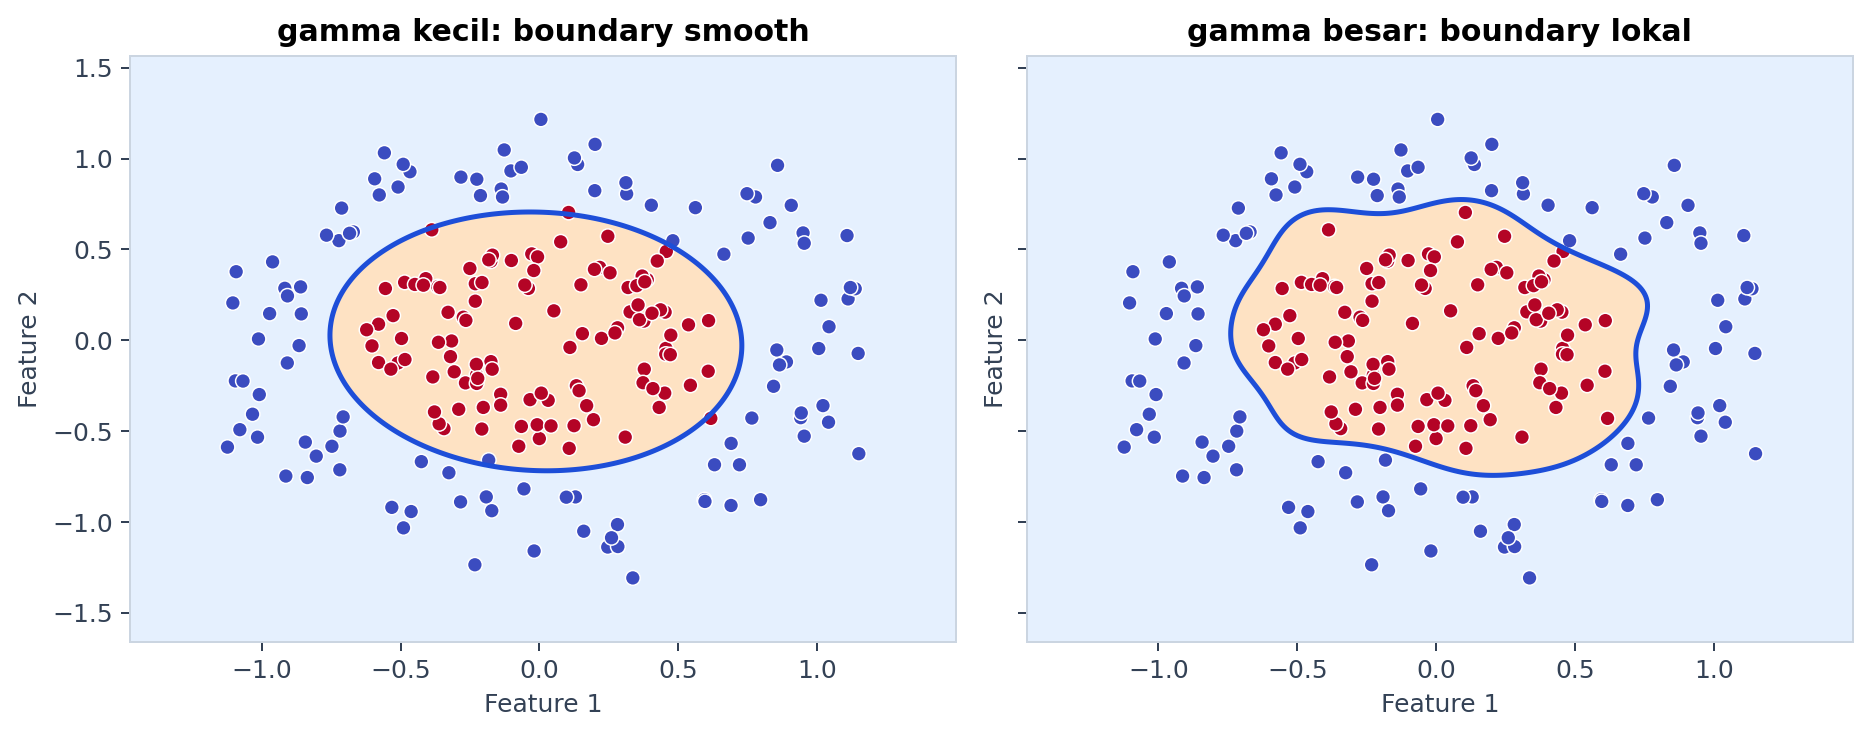
\includegraphics[width=0.98\textwidth]{figures/03_rbf_gamma_effect.png}
\caption{Efek parameter \code{gamma} pada RBF kernel. Gamma kecil menghasilkan boundary smooth, sedangkan gamma besar membuat boundary sangat lokal dan mudah overfit.}
\end{figure}

\section{Parameter Penting SVC}

\begin{table}[H]
\centering
\rowcolors{2}{softOrange}{white}
\begin{tabularx}{\textwidth}{>{\bfseries}lXX}
\rowcolor{softOrange}
Parameter & Berlaku Untuk & Makna \\
\toprule
\code{C} & semua kernel & Penalty untuk training error dan margin violation. \\
\code{kernel} & semua & Jenis similarity function yang dipakai. \\
\code{gamma} & rbf, poly, sigmoid & Seberapa jauh pengaruh satu training point. \\
\code{degree} & poly & Derajat polynomial kernel. \\
\code{coef0} & poly, sigmoid & Independent term dalam kernel. \\
\code{class\_weight} & classification & Bobot class, berguna untuk imbalanced data. \\
\code{probability} & SVC & Mengaktifkan probability estimate, tetapi training menjadi lebih mahal. \\
\bottomrule
\end{tabularx}
\caption{Parameter penting dalam \code{sklearn.svm.SVC}.}
\end{table}

\infobox{softGreen}{\textbf{Rule of thumb.} Mulai dari \code{Pipeline(StandardScaler(), SVC(kernel="rbf"))}, lalu tune \code{C} dan \code{gamma}. Jika dataset sangat besar atau text-like, pertimbangkan \code{LinearSVC} atau \code{SGDClassifier}.}

\section{Mencari Parameter Optimal}

\subsection{Grid Search}

Grid Search mencoba semua kombinasi parameter dalam grid. Untuk SVC, grid yang umum adalah kombinasi \code{kernel}, \code{C}, dan \code{gamma}. Pada pipeline, parameter ditulis dengan pola \code{step\_\_parameter}, misalnya \code{svc\_\_C}.

\begin{lstlisting}[language=Python]
from sklearn.model_selection import GridSearchCV
from sklearn.pipeline import Pipeline
from sklearn.preprocessing import StandardScaler
from sklearn.svm import SVC

pipe = Pipeline([
    ("scaler", StandardScaler()),
    ("svc", SVC())
])

param_grid = [
    {"svc__kernel": ["linear"], "svc__C": [0.1, 1, 10, 100]},
    {"svc__kernel": ["rbf"], "svc__C": [0.1, 1, 10, 100],
     "svc__gamma": [0.001, 0.01, 0.1, 1]},
]

search = GridSearchCV(pipe, param_grid, cv=5,
                      scoring="accuracy", n_jobs=-1)
search.fit(X_train, y_train)
\end{lstlisting}

\begin{figure}[H]
\centering
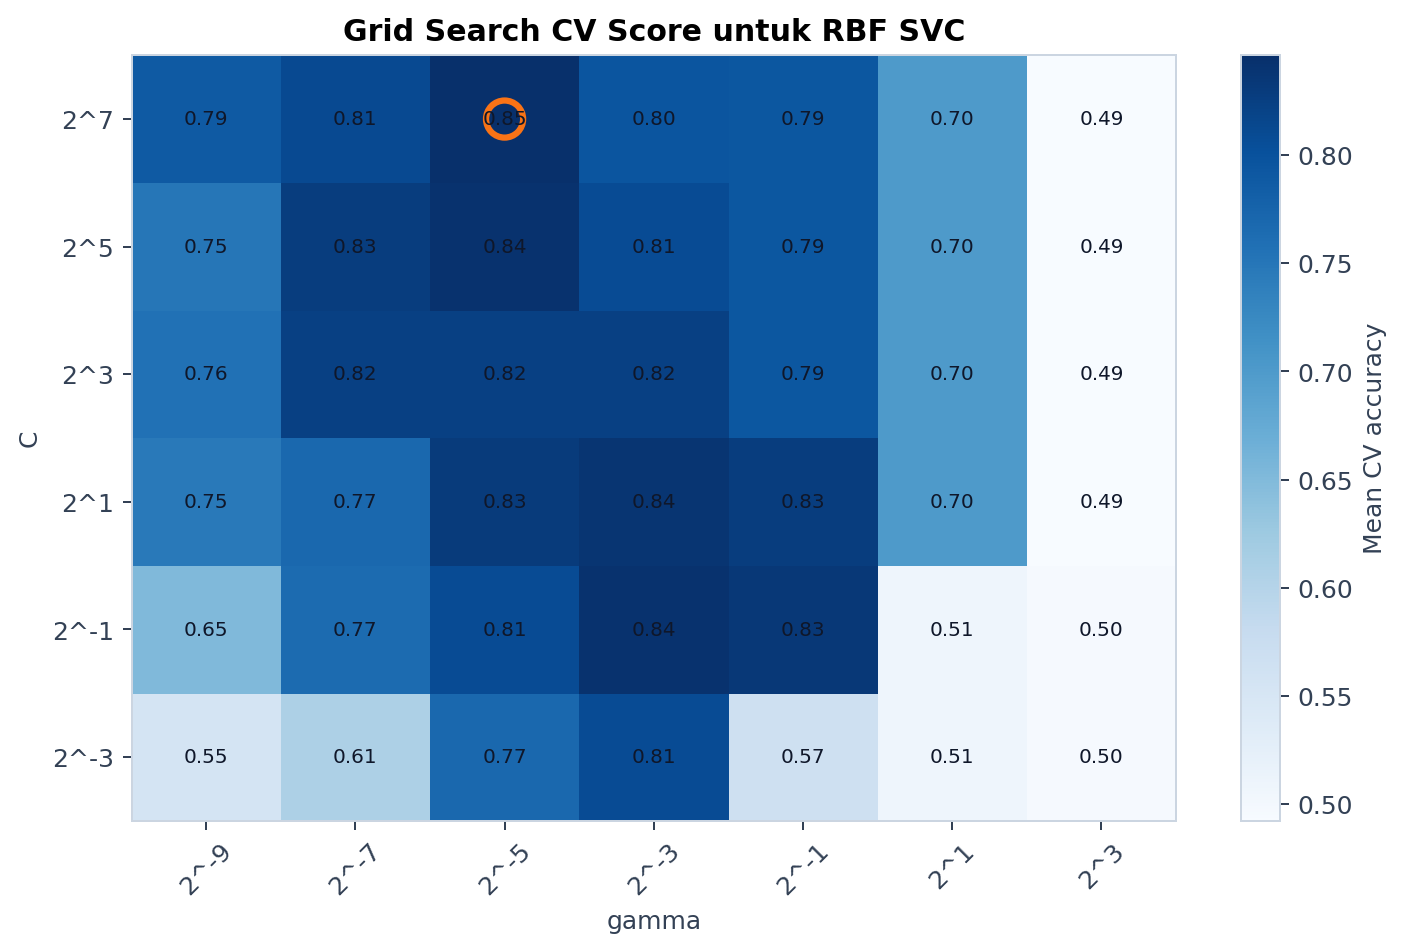
\includegraphics[width=0.86\textwidth]{figures/04_grid_search_heatmap.png}
\caption{Contoh heatmap Grid Search untuk RBF SVC. Nilai \code{C} dan \code{gamma} dicoba pada skala log, lalu kombinasi terbaik dipilih berdasarkan cross-validation score.}
\end{figure}

\subsection{Random Search}

Random Search sampling kombinasi parameter dari distribusi. Ini cocok ketika search space besar dan kita ingin mengontrol budget komputasi dengan \code{n\_iter}.

\begin{lstlisting}[language=Python]
from scipy.stats import loguniform
from sklearn.model_selection import RandomizedSearchCV

param_dist = {
    "svc__kernel": ["rbf"],
    "svc__C": loguniform(1e-3, 1e3),
    "svc__gamma": loguniform(1e-4, 1e1),
}

search = RandomizedSearchCV(
    pipe, param_distributions=param_dist,
    n_iter=50, cv=5, scoring="accuracy",
    n_jobs=-1, random_state=42
)
\end{lstlisting}

\subsection{Optuna}

Optuna mendefinisikan search space secara Pythonic. Cocok ketika parameter bersifat conditional, misalnya \code{gamma} hanya dicoba untuk kernel tertentu.

\begin{lstlisting}[language=Python]
import optuna
from sklearn.model_selection import cross_val_score

def objective(trial):
    C = trial.suggest_float("C", 1e-3, 1e3, log=True)
    gamma = trial.suggest_float("gamma", 1e-4, 1e1, log=True)

    model = Pipeline([
        ("scaler", StandardScaler()),
        ("svc", SVC(kernel="rbf", C=C, gamma=gamma))
    ])

    scores = cross_val_score(model, X_train, y_train,
                             cv=5, scoring="accuracy")
    return scores.mean()

study = optuna.create_study(direction="maximize")
study.optimize(objective, n_trials=50)
\end{lstlisting}

\begin{table}[H]
\centering
\rowcolors{2}{softBlue}{white}
\begin{tabularx}{\textwidth}{>{\bfseries}lXX}
\rowcolor{tableHead}
Metode & Kelebihan & Kekurangan \\
\toprule
Grid Search & Exhaustive dan mudah dijelaskan. & Mahal jika kombinasi banyak. \\
Random Search & Budget fleksibel dan cocok untuk parameter continuous. & Bisa miss region bagus jika trial sedikit. \\
Optuna & Fleksibel, conditional, dan trial-based. & Perlu library tambahan dan konsep lebih advanced. \\
\bottomrule
\end{tabularx}
\caption{Perbandingan metode hyperparameter tuning untuk SVC.}
\end{table}

\section{Practical Workflow dan Common Mistakes}

Workflow yang direkomendasikan:

\begin{enumerate}[leftmargin=*]
    \item Split data menjadi training dan testing set.
    \item Buat pipeline \code{StandardScaler + SVC}.
    \item Tentukan metric sesuai problem, misalnya accuracy, F1, recall, ROC-AUC, atau balanced accuracy.
    \item Jalankan baseline model.
    \item Tune parameter dengan Grid Search, Random Search, atau Optuna pada training set.
    \item Refit model terbaik pada training set.
    \item Evaluasi final pada test set.
\end{enumerate}

\begin{table}[H]
\centering
\rowcolors{2}{softOrange}{white}
\begin{tabularx}{\textwidth}{>{\bfseries}lXX}
\rowcolor{softOrange}
Mistake & Dampak & Fix \\
\toprule
Tidak scaling fitur & Feature range besar mendominasi kernel. & Pakai \code{StandardScaler} dalam \code{Pipeline}. \\
Tuning di test set & Evaluasi final terlalu optimis. & Tune dengan cross-validation pada train set. \\
Grid terlalu sempit & Parameter terbaik tidak ditemukan. & Gunakan log-spaced range luas dulu. \\
\code{C} terlalu besar & Boundary overfit. & Coba \code{C} lebih kecil. \\
\code{gamma} terlalu besar & Boundary terlalu lokal. & Coba \code{gamma} lebih kecil. \\
Accuracy untuk imbalance & Metric misleading. & Pakai F1, recall, ROC-AUC, atau balanced accuracy. \\
\bottomrule
\end{tabularx}
\caption{Kesalahan umum saat menggunakan SVC dan cara menghindarinya.}
\end{table}

\section{Latihan}

\begin{enumerate}[leftmargin=*]
    \item Diberikan dua decision boundary yang sama-sama memisahkan class. Jelaskan boundary mana yang lebih baik menurut SVM dan kenapa.
    \item Jelaskan efek kombinasi \code{C} kecil-besar dan \code{gamma} kecil-besar terhadap boundary RBF SVC.
    \item Buat pipeline \code{StandardScaler -> SVC}, lalu lakukan \code{GridSearchCV} untuk kernel linear dan RBF.
    \item Jika dataset memiliki class ratio 95:5, kenapa accuracy tidak cukup? Metric apa yang lebih cocok?
\end{enumerate}

\section*{Referensi}

\begin{itemize}[leftmargin=*]
    \item Cortes, C. \& Vapnik, V. (1995). \textit{Support-Vector Networks}. Machine Learning, 20, 273--297.
    \item Boser, B. E., Guyon, I. M. \& Vapnik, V. N. (1992). \textit{A Training Algorithm for Optimal Margin Classifiers}.
    \item Hsu, C.-W., Chang, C.-C. \& Lin, C.-J. (2025). \textit{A Practical Guide to Support Vector Classification}.
    \item Chang, C.-C. \& Lin, C.-J. (2011). \textit{LIBSVM: A Library for Support Vector Machines}.
    \item Bergstra, J. \& Bengio, Y. (2012). \textit{Random Search for Hyper-Parameter Optimization}.
    \item scikit-learn SVM User Guide: \url{https://scikit-learn.org/stable/modules/svm.html}
    \item scikit-learn hyperparameter tuning: \url{https://scikit-learn.org/stable/modules/grid_search.html}
    \item Optuna documentation: \url{https://optuna.readthedocs.io/}
\end{itemize}

\end{document}
